\documentclass{article}
\usepackage{amssymb,amsmath}
\usepackage{ifxetex,ifluatex}
\ifxetex
  \usepackage{fontspec,xltxtra,xunicode}
  \defaultfontfeatures{Mapping=tex-text,Scale=MatchLowercase}
\else
  \ifluatex
    \usepackage{fontspec}
    \defaultfontfeatures{Mapping=tex-text,Scale=MatchLowercase}
  \else
    \usepackage[utf8]{inputenc}
  \fi
\fi
\usepackage{ctable}
\usepackage{float} % provides the H option for float placement
\usepackage{graphicx}
% We will generate all images so they have a width \maxwidth. This means
% that they will get their normal width if they fit onto the page, but
% are scaled down if they would overflow the margins.
\makeatletter
\def\maxwidth{\ifdim\Gin@nat@width>\linewidth\linewidth
\else\Gin@nat@width\fi}
\makeatother
\let\Oldincludegraphics\includegraphics
\renewcommand{\includegraphics}[1]{\Oldincludegraphics[width=\maxwidth]{#1}}
\ifxetex
  \usepackage[setpagesize=false, % page size defined by xetex
              unicode=false, % unicode breaks when used with xetex
              xetex]{hyperref}
\else
  \usepackage[unicode=true]{hyperref}
\fi
\hypersetup{breaklinks=true, pdfborder={0 0 0}}
\setlength{\parindent}{0pt}
\setlength{\parskip}{6pt plus 2pt minus 1pt}
\setlength{\emergencystretch}{3em}  % prevent overfull lines
\setcounter{secnumdepth}{0}

\title{Correlations}
\author{Rapport package team @ https://github.com/aL3xa/rapport}
\date{2011--04--26 20:25 CET}

\begin{document}
\maketitle

\subsection{Description}

This template will return the correlation matrix of supplied numerical
variables.

\subsubsection{Variable description}

3 variables provided.

The highest correlation coefficient (0.2364) is between \emph{edu} and
\emph{age} and the lowest (--0.049) is between \emph{leisure} and
\emph{age}. It seems that the strongest association (r=0.2364) is
between \emph{edu} and \emph{age}.

Higly correlated (r \textless{} 0.7 or r \textgreater{} 0.7) variables:
-

Uncorrelated (--0.2 \textless{} r \textless{} 0.2) variables:

\begin{itemize}
\item
  \emph{age} and \emph{leisure}
\item
  \emph{edu} and \emph{leisure}
\end{itemize}
\paragraph{Correlation matrix}

\ctable[pos = H, center, botcap]{llll}
{% notes
}
{% rows
\FL
 & \textbf{age} & \textbf{edu} & \textbf{leisure}
\ML
age &  & 0.2364 *** --0. & 0490
\\\noalign{\medskip}
edu & 0.2364 *** & 0.1 & 714 ***
\\\noalign{\medskip}
leisure & --0.0490 & 0.1714 *** & 
\LL
}

\begin{figure}[htbp]
\centering
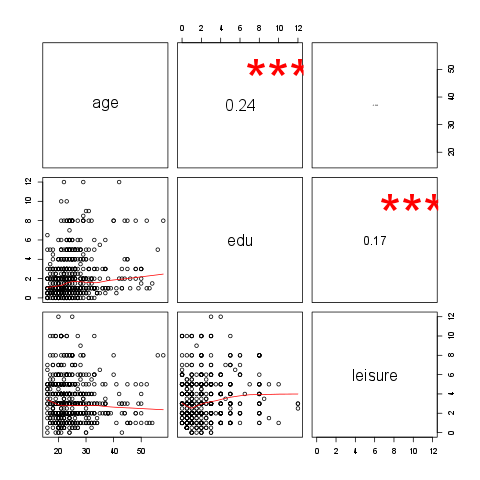
\includegraphics{f4c6c0be648793b84a85d267c1a8ecd3.png}
\caption{}
\end{figure}

\subsection{Description}

This template will return the correlation matrix of supplied numerical
variables.

\subsubsection{Variable description}

11 variables provided.

The highest correlation coefficient (0.902) is between \emph{disp} and
\emph{cyl} and the lowest (--0.8677) is between \emph{wt} and
\emph{mpg}. It seems that the strongest association (r=0.902) is between
\emph{disp} and \emph{cyl}.

Higly correlated (r \textless{} 0.7 or r \textgreater{} 0.7) variables:

\begin{itemize}
\item
  \emph{mpg} and \emph{cyl}
\item
  \emph{mpg} and \emph{disp}
\item
  \emph{cyl} and \emph{disp}
\item
  \emph{mpg} and \emph{hp}
\item
  \emph{cyl} and \emph{hp}
\item
  \emph{disp} and \emph{hp}
\item
  \emph{disp} and \emph{drat}
\item
  \emph{mpg} and \emph{wt}
\item
  \emph{cyl} and \emph{wt}
\item
  \emph{disp} and \emph{wt}
\item
  \emph{drat} and \emph{wt}
\item
  \emph{hp} and \emph{qsec}
\item
  \emph{cyl} and \emph{vs}
\item
  \emph{disp} and \emph{vs}
\item
  \emph{hp} and \emph{vs}
\item
  \emph{qsec} and \emph{vs}
\item
  \emph{drat} and \emph{am}
\item
  \emph{am} and \emph{gear}
\item
  \emph{hp} and \emph{carb}
\end{itemize}
Uncorrelated (--0.2 \textless{} r \textless{} 0.2) variables:

\begin{itemize}
\item
  \emph{drat} and \emph{qsec}
\item
  \emph{wt} and \emph{qsec}
\item
  \emph{vs} and \emph{am}
\item
  \emph{hp} and \emph{gear}
\item
  \emph{drat} and \emph{carb}
\item
  \emph{am} and \emph{carb}
\end{itemize}
\paragraph{Correlation matrix}

\ctable[pos = H, center, botcap]{llllllllllll}
{% notes
}
{% rows
\FL
 & \textbf{mpg} & \textbf{cyl} & \textbf{disp} & \textbf{hp} & \textbf{drat} & \textbf{wt} & \textbf{qsec} & \textbf{vs} & \textbf{am} & \textbf{gear} & \textbf{carb}
\ML
mpg &  & --0.8522 *** --0. & 8476 *** --0.776 & 2 *** 0.6812 * & **
--0.8677 ** & * 0.4187 * & 0.6640 *** 0 & .5998 *** 0.48 & 03 **
--0.550 & 9 ** & 
\\\noalign{\medskip}
cyl & --0.8522 *** & 0.9 & 020 *** 0.8324 & *** --0.6999
\textbackslash{} & *** 0.7825 **\textbackslash{} & * --0.5912
*** & --0.8108 *** --0. & 5226 ** --0.49 & 27 ** 0.5270 & ** & 
\\\noalign{\medskip}
disp & --0.8476 *** 0.9 & 020 *** & 0.7909 & *** --0.7102
\textbackslash{} & *** 0.8880 **\textbackslash{} & * --0.4337
* & --0.7104 *** - & 0.5912 *** --0.5 & 556 *** 0.3950 & * & 
\\\noalign{\medskip}
hp & --0.7762 *** 0.8 & 324 *** 0.7909 & *** & --0.4488
\textbackslash{} & ** 0.6587 ** & * --0.7082 *** & --0.7231 ***
--0 & .2432 --0 & .1257 0. & 7498 *** & 
\\\noalign{\medskip}
drat & 0.6812 *** --0. & 6999 *** --0.710 & 2 *** --0.4488
\textbackslash{} & ** & --0.7124 *\textbackslash{} & ** 0.0912 & 0.4403
* & 0.7127 *** & 0.6996 *** --0. & 0908 & 
\\\noalign{\medskip}
wt & --0.8677 *** 0.7 & 825 *** 0.8880 & *** 0.6587 * & ** --0.7124
** & * & --0.1747 & --0.5549 *** & --0.6925 *** --0. & 5833 ***
0.4276 & * & 
\\\noalign{\medskip}
qsec & 0.4187 * - & 0.5912 *** --0.4 & 337 * --0.70 & 82 ***
0.0912 & --0.1747 &  & 0.7445 \textbackslash{} & ***
--0.2299 & --0.2127 & --0.6562 *\textbackslash{} & **
\\\noalign{\medskip}
vs & 0.6640 *** --0. & 8108 *** --0.710 & 4 *** --0.7231
\textbackslash{} & *** 0.4403 * & --0.5549 **\textbackslash{} & * 0.7445
*** & 0 & .1683 0 & .2060 - & 0.5696 *** & 
\\\noalign{\medskip}
am & 0.5998 *** --0. & 5226 ** --0.59 & 12 *** --0.2432 & 0.7127
\textbackslash{} & *** --0.6925 *\textbackslash{} & **
--0.2299 & 0.1683 &  & 0.7941 *** & 0.0575 & 
\\\noalign{\medskip}
gear & 0.4803 ** --0 & .4927 ** --0.5 & 556 *** --0.1257 & 0.6996 & ***
--0.5833 * & ** --0.2127 & 0.2060 & 0.7941 *** &  & 0.2741 & 
\\\noalign{\medskip}
carb & --0.5509 ** 0. & 5270 ** 0.39 & 50 * 0.749 & 8 ***
--0.0908 & 0.4276 \textbackslash{} & * --0.6562 \textbackslash{} & ***
--0.5696 ** & * 0.0575 & 0.2741 &  & 
\LL
}

\begin{figure}[htbp]
\centering
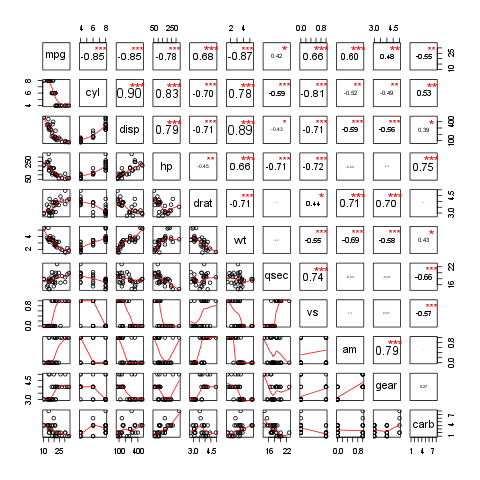
\includegraphics{ce42e944b62284a3bebf2101155af100.png}
\caption{}
\end{figure}

\end{document}
